\documentclass[spanish, fleqn]{scrartcl}
\usepackage[utf8]{inputenc}
\usepackage{babel}
\usepackage[paper=a4paper, top=2cm, left=2cm, right=2cm]{geometry}
\usepackage{tikz}
\usepackage{CIACcustom}
\usepackage{fourier}
\usepackage{amsmath, amsthm}
\usepackage{listings}
\usepackage{multicol}
\usepackage{fancyhdr}
\usepackage[urlcolor=blue, colorlinks]{hyperref}
\usepackage{booktabs,tabularx}
\usepackage{float}

\newcolumntype{L}[1]{>{\hsize=#1\hsize\raggedright\arraybackslash}X}%
\newcolumntype{R}[1]{>{\hsize=#1\hsize\raggedleft\arraybackslash}X}%
\newcolumntype{C}[2]{>{\hsize=#1\hsize\columncolor{#2}\centering\arraybackslash}X}%

\pagestyle{fancy}
\fancyhf{}
\rhead{\pgfimage[width=2.5cm]{imagenes/logo-ciac.png}}
\chead{
  Apoyos intensivos Pauta N° 2\\
  IWI-131 Semestre I-2016 \\
  CIAC Casa Central
}
\lhead{\pgfimage[width=2.5cm]{imagenes/logo-usm.jpg}}
\rfoot{\LaTeXe / CIAC 2016}
\lfoot{\thepage}

\renewcommand{\ttdefault}{pcr}

%%% listings settings:
\definecolor{bggray}{rgb}{0.95,0.95,0.95}
\lstdefinestyle{consola}{
  backgroundcolor=\color{bggray},
  basicstyle=\small\ttfamily,
  frame=single,
  moredelim=[is][\bfseries]{[*}{*]},
  xrightmargin=5pt
}

\lstdefinestyle{mypy}{
  language=python,
  backgroundcolor=\color{bggray},
  basicstyle=\ttfamily\small\color{orange!70!black},
  frame=L,
  keywordstyle=\bfseries\color{green!40!black},
  commentstyle=\itshape\color{purple!40!black},
  identifierstyle=\color{blue},
  stringstyle=\color{red},
  numbers=left,
  showstringspaces=false,
  xrightmargin=5pt,
  xleftmargin=10pt
}

\newtheorem{CIACdef}{Definición}

\begin{document}
\vspace*{.3cm}
\section{Contabilidad Básica}

Un antiguo ingeniero comercial que olvidó como programar le pide ayuda a usted en el balance de cuentas de su empresa. Algunas cuentas se corrigen monetariamente en base al IPC y otras se deprecian.

Se tienen dos archivos \texttt{archivos.txt} y \texttt{pasivos.txt}. Dentro de ellos hay dos tipos de formas, \texttt{cuenta; indicacion; monto} y \texttt{cuenta; indicacion; valor\_residual; vida\_útil; monto}, esta última es para bienes que se deprecian.

\begin{figure}[h]
    \centering
    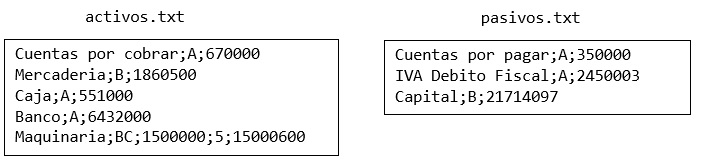
\includegraphics{Imagenes/imagen1.jpg}
\end{figure}

Las indicaciones son:
\begin{itemize}
    \item[A:] No existe ningún cambio
    \item[B:] Hay ajuste monetario por IPC
    \item[C:] Se deprecia
\end{itemize}

Afortunadamente para usted, este ingeniero aún no necesita depreciar sus bienes. 
Se tiene un diccionario \texttt{valores\_IPC} cuyas llaves son tuplas de fechas (año,mes) y sus valores son los puntos del IPC

\begin{lstlisting}[style=consola]
valores_IPC={
(2016,1):111.39, (2016,2):111.70, (2016,3):112.13,
(2016,4):112.49, (2016,5):112.75, (2015,1):106.30, (2015,2):106.68,
(2015,3):107.35, (2015,4):107.97, (2015,5):108.16, (2015,6):108.68,
(2015,7):109.14, (2015,8):109.88, (2015,9):110.44, (2015,10):110.89,
(2015,11):110.86, (2015,12):110.87}
\end{lstlisting}

Cree las funciones:
\begin{itemize}
    \item[a.] \texttt{total(archivo)} que recibiendo un string de un archivo retorne un entero con la suma total de los montos indicados en el archivo.
    \item[b.] \texttt{correccion(archivo,actual,inicial)} que reciba un string con el nombre del archivo a corregir y dos tuplas con el mes actual e inicial de forma (año,mes). Esta función debe actualizar el monto siguiendo las indicaciones dadas. Se entenderá que para corregir un monto se multiplicará por la razón de los valores del IPC de la fecha actual y la fecha inicial.
\end{itemize}

\paragraph{Aclaraciones} Lo del ingeniero comercial es mentira. La corrección monetaria se calcula de otra forma, pero para efectos de algoritmo se ha simplificado.

\end{document}